\documentclass[si.tex]{subfiles}

\begin{document}


\begin{comment}
cd ./code/Synthetic
. ./recover.sh

#Parameters:
#
#\begin{itemize}
#  \item \texttt{GRID}: number of discrete orientation bins covering $[0,360)$°.
#  \item \texttt{h\_deg}: finite‐difference step $h$ in degrees (used to compute choice probabilities).
#  \item \texttt{smooth\_sigma}: Gaussian kernel standard deviation for optional smoothing of $\sqrt{J}(\theta)$.
#  \item \texttt{FIT}: name of the data file 
#\end{itemize}
\end{comment}


%\textcolor{red}{TODO}
%
%    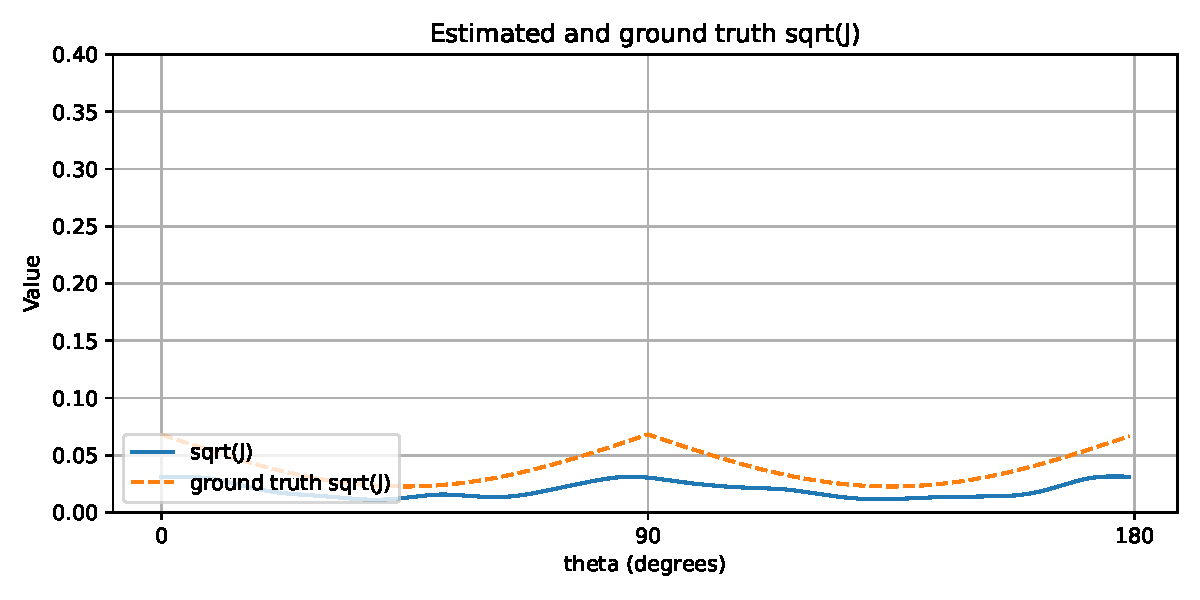
\includegraphics[width=0.2\textwidth]{figures/recover_encoding.py_SimulateSynthetic_Parameterized_OtherNoiseLevels_Grid_VarySize.py_180_2_2_N40000_UNIFORM_STEEPPERIODIC.txt_180_4.0_6.0_sqrtJ.pdf}
%    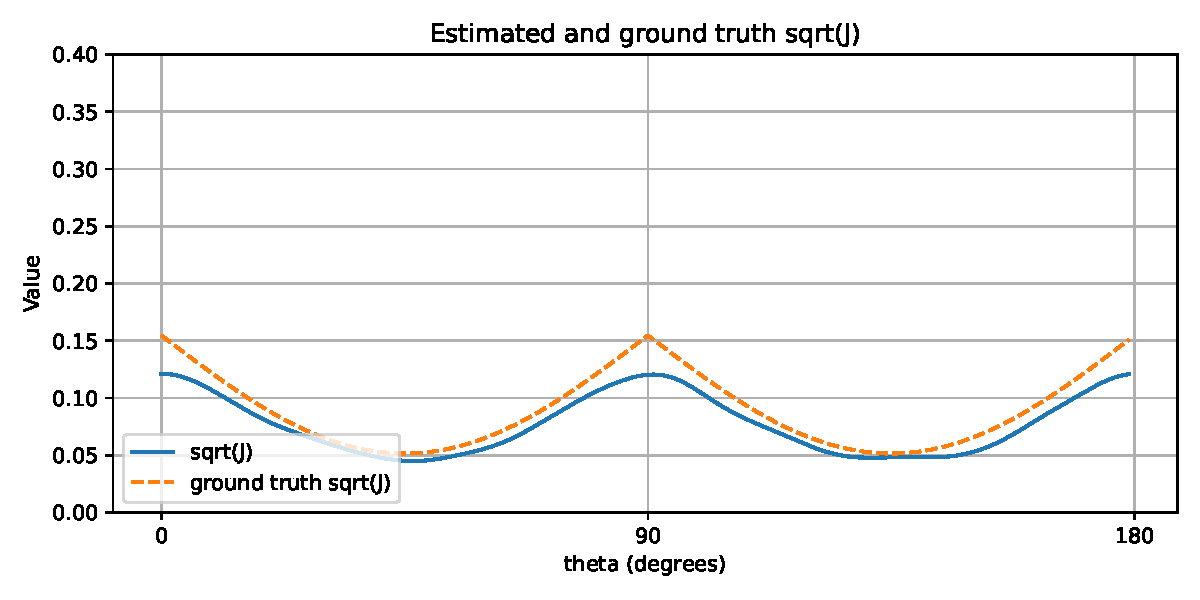
\includegraphics[width=0.2\textwidth]{figures/recover_encoding.py_SimulateSynthetic_Parameterized_OtherNoiseLevels_Grid_VarySize.py_180_2_3_N40000_UNIFORM_STEEPPERIODIC.txt_180_4.0_6.0_sqrtJ.pdf}
%    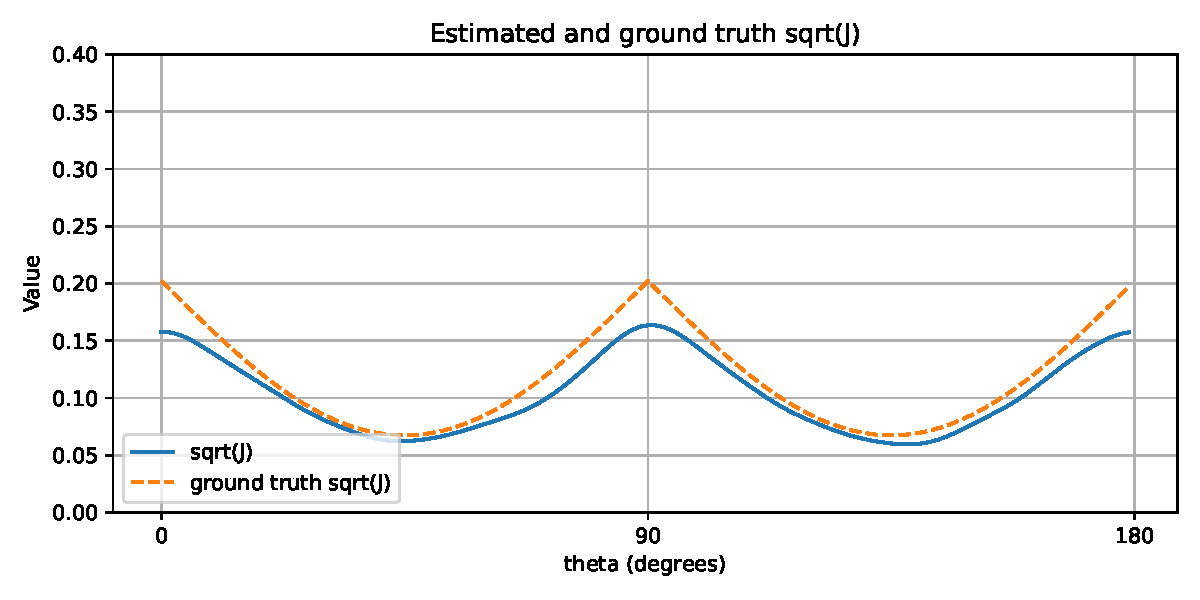
\includegraphics[width=0.2\textwidth]{figures/recover_encoding.py_SimulateSynthetic_Parameterized_OtherNoiseLevels_Grid_VarySize.py_180_2_4_N40000_UNIFORM_STEEPPERIODIC.txt_180_4.0_6.0_sqrtJ.pdf}
%    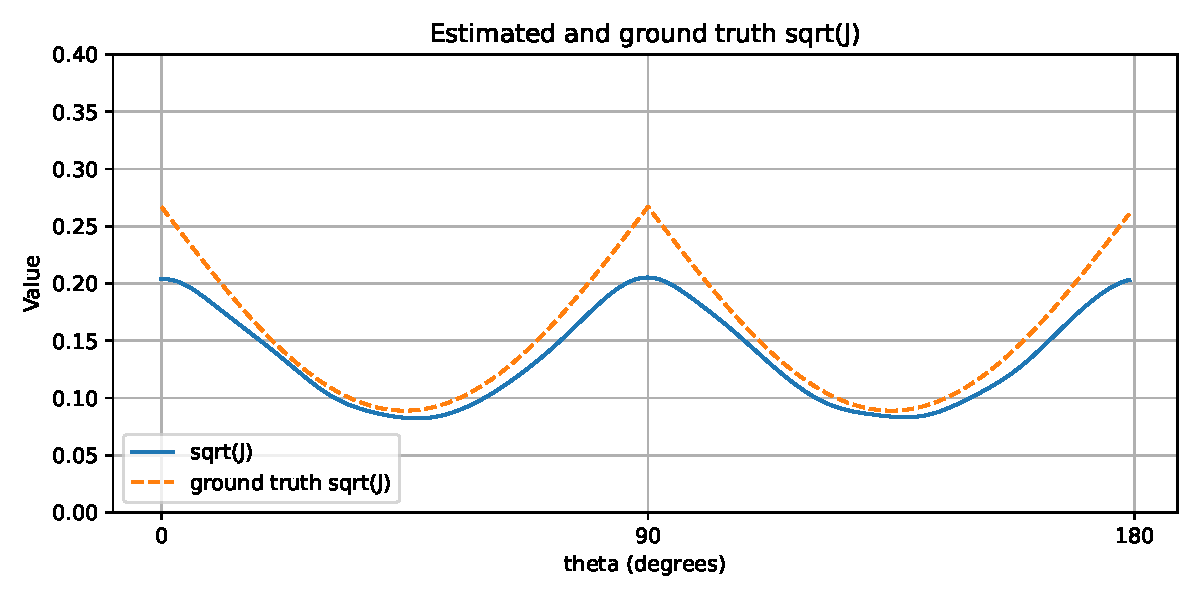
\includegraphics[width=0.2\textwidth]{figures/recover_encoding.py_SimulateSynthetic_Parameterized_OtherNoiseLevels_Grid_VarySize.py_180_2_5_N40000_UNIFORM_STEEPPERIODIC.txt_180_4.0_6.0_sqrtJ.pdf}

\begin{figure}[ht]
  \centering

High Noise

  \begin{minipage}[b]{0.45\textwidth}
    \centering
    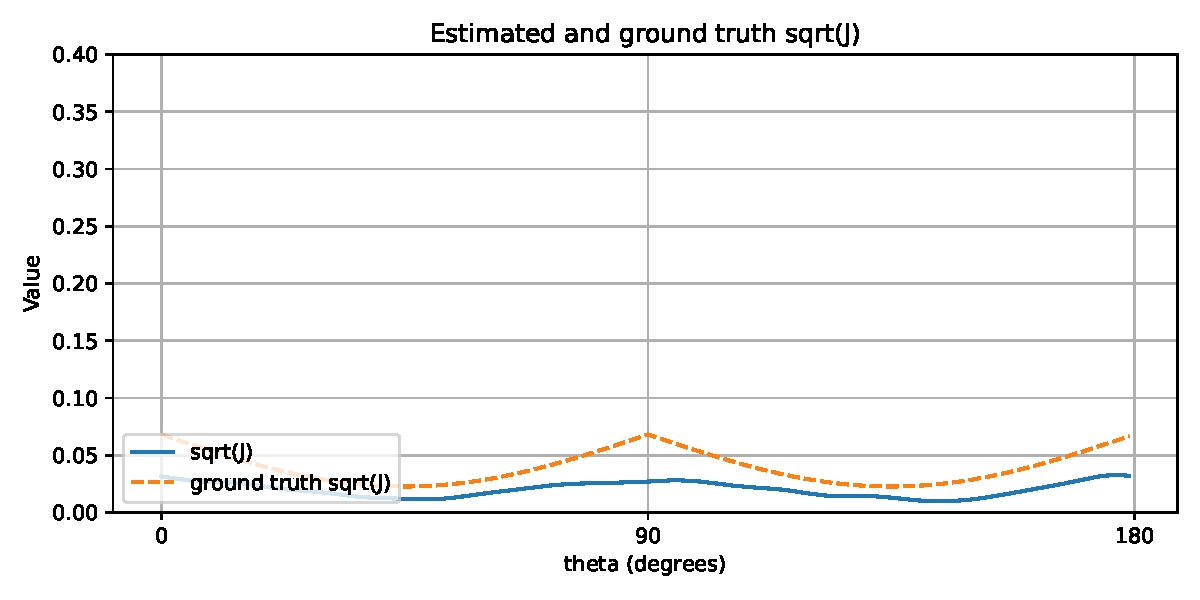
\includegraphics[width=\textwidth]{figures/recover_encoding.py_SimulateSynthetic_Parameterized_OtherNoiseLevels_Grid_VarySize.py_180_2_2_N40000_STEEPPERIODIC_STEEPPERIODIC.txt_180_4.0_6.0_sqrtJ.pdf}
  \end{minipage}
  \hfill
  \begin{minipage}[b]{0.45\textwidth}
    \centering
    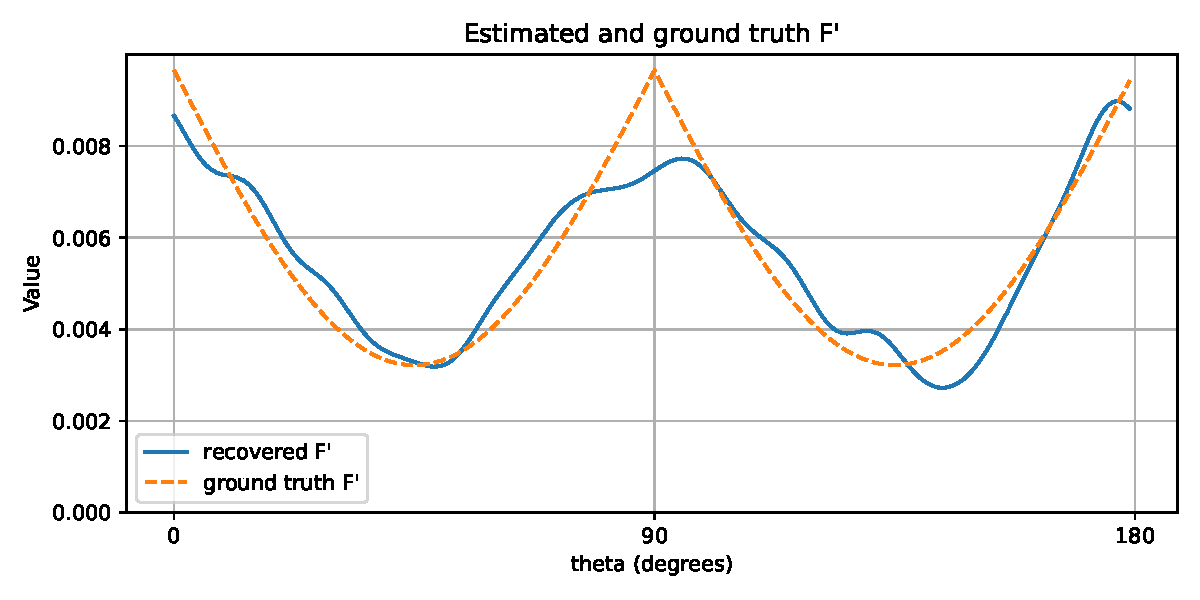
\includegraphics[width=\textwidth]{figures/recover_encoding.py_SimulateSynthetic_Parameterized_OtherNoiseLevels_Grid_VarySize.py_180_2_2_N40000_STEEPPERIODIC_STEEPPERIODIC.txt_180_4.0_6.0_Fprime.pdf}
  \end{minipage}

Mid-High Noise

  \begin{minipage}[b]{0.45\textwidth}
    \centering
    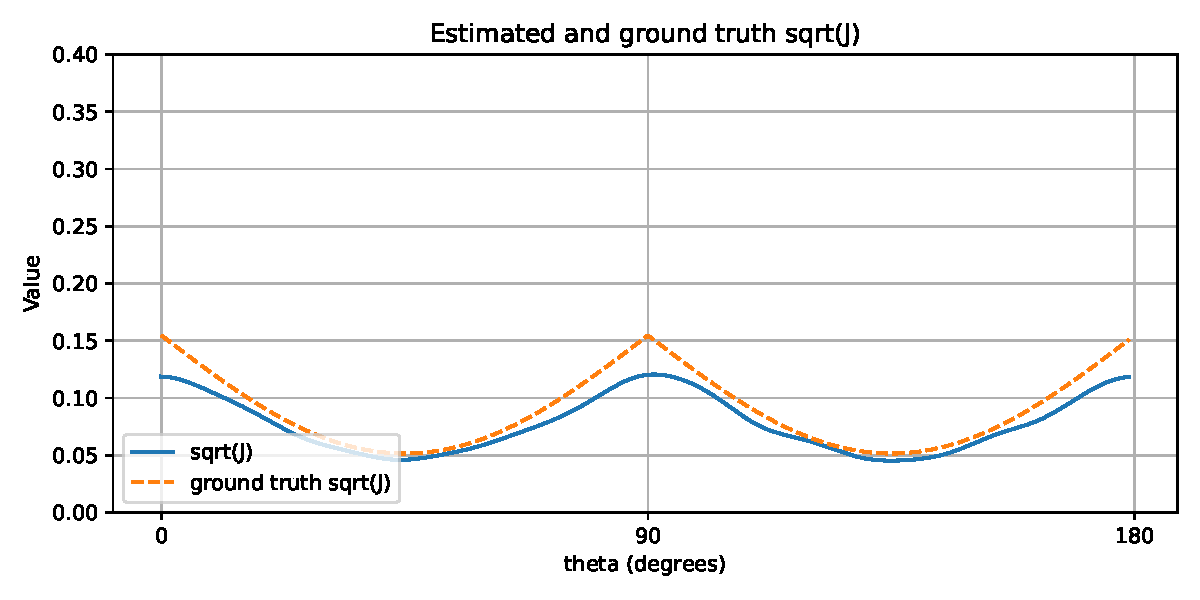
\includegraphics[width=\textwidth]{figures/recover_encoding.py_SimulateSynthetic_Parameterized_OtherNoiseLevels_Grid_VarySize.py_180_2_3_N40000_STEEPPERIODIC_STEEPPERIODIC.txt_180_4.0_6.0_sqrtJ.pdf}
  \end{minipage}
  \hfill
  \begin{minipage}[b]{0.45\textwidth}
    \centering
    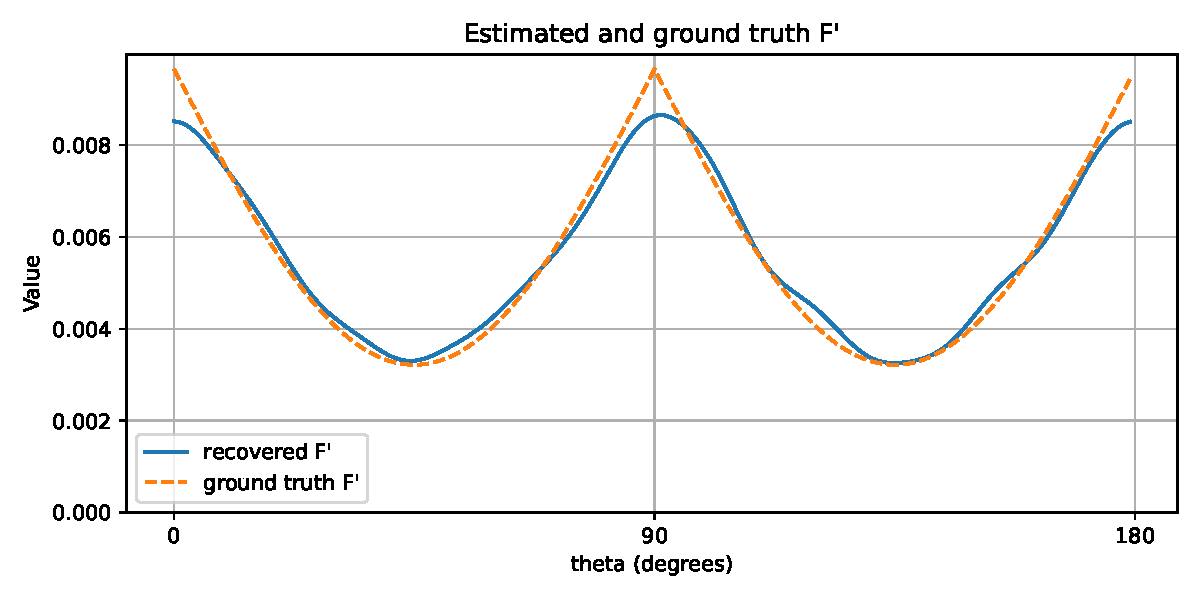
\includegraphics[width=\textwidth]{figures/recover_encoding.py_SimulateSynthetic_Parameterized_OtherNoiseLevels_Grid_VarySize.py_180_2_3_N40000_STEEPPERIODIC_STEEPPERIODIC.txt_180_4.0_6.0_Fprime.pdf}
  \end{minipage}

Mid-Low Noise

  \begin{minipage}[b]{0.45\textwidth}
    \centering
    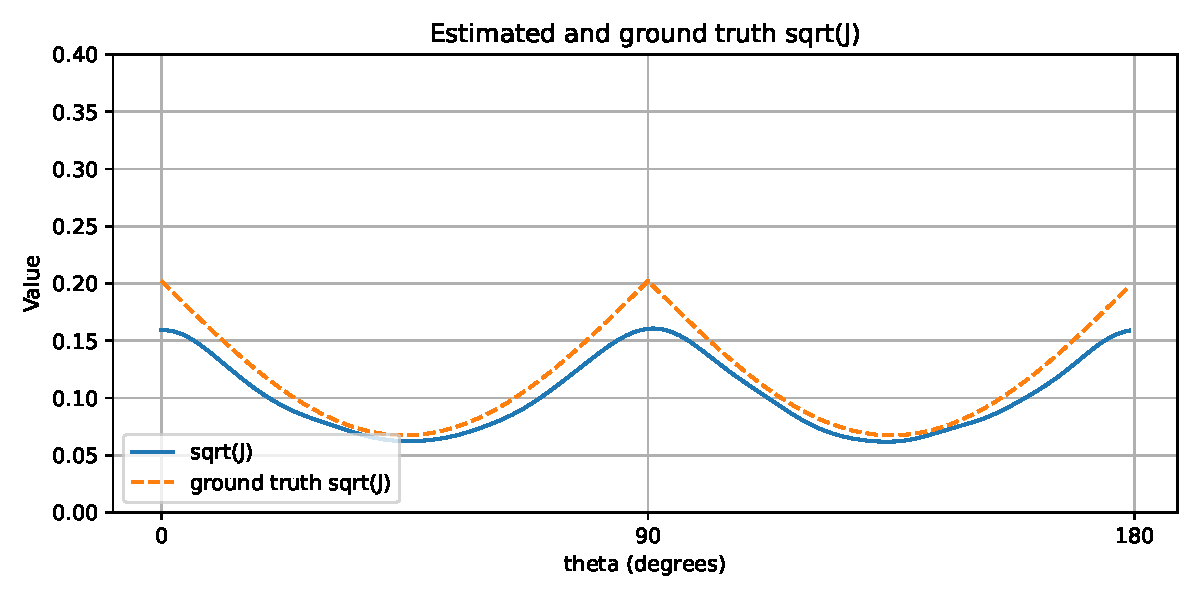
\includegraphics[width=\textwidth]{figures/recover_encoding.py_SimulateSynthetic_Parameterized_OtherNoiseLevels_Grid_VarySize.py_180_2_4_N40000_STEEPPERIODIC_STEEPPERIODIC.txt_180_4.0_6.0_sqrtJ.pdf}
  \end{minipage}
  \hfill
  \begin{minipage}[b]{0.45\textwidth}
    \centering
    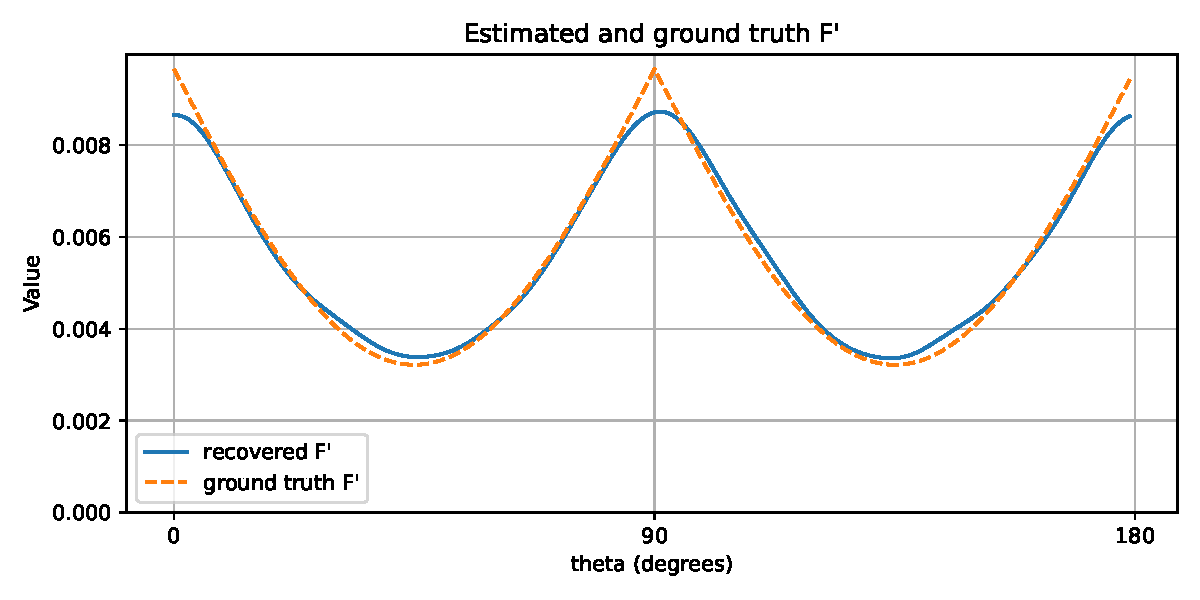
\includegraphics[width=\textwidth]{figures/recover_encoding.py_SimulateSynthetic_Parameterized_OtherNoiseLevels_Grid_VarySize.py_180_2_4_N40000_STEEPPERIODIC_STEEPPERIODIC.txt_180_4.0_6.0_Fprime.pdf}
  \end{minipage}

Low Noise

  \begin{minipage}[b]{0.45\textwidth}
    \centering
    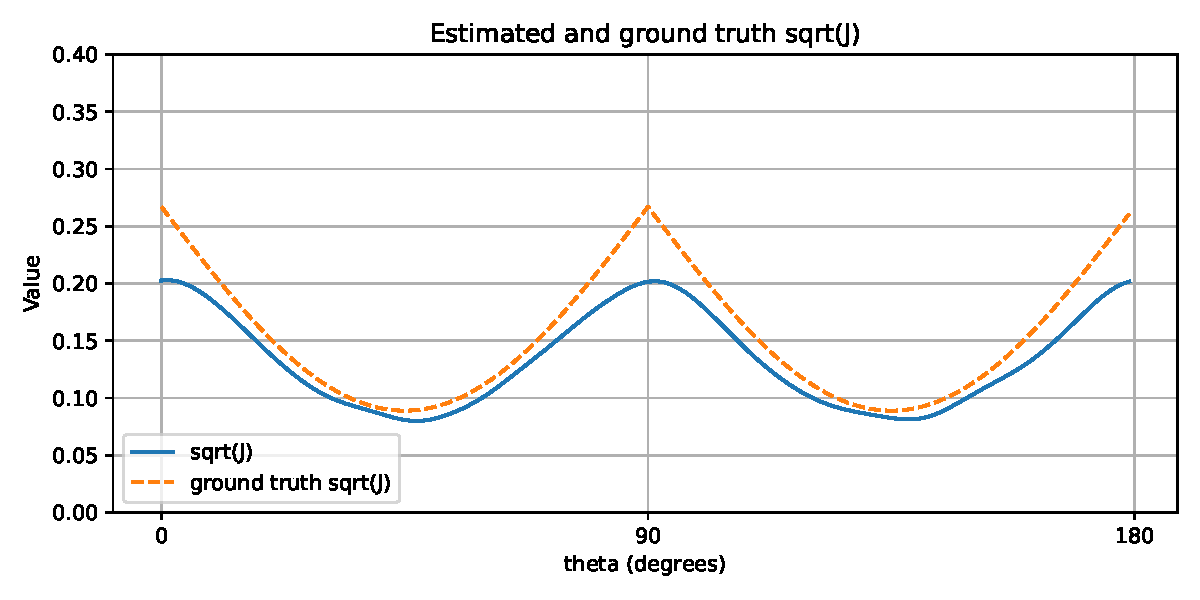
\includegraphics[width=\textwidth]{figures/recover_encoding.py_SimulateSynthetic_Parameterized_OtherNoiseLevels_Grid_VarySize.py_180_2_5_N40000_STEEPPERIODIC_STEEPPERIODIC.txt_180_4.0_6.0_sqrtJ.pdf}
  \end{minipage}
  \hfill
  \begin{minipage}[b]{0.45\textwidth}
    \centering
    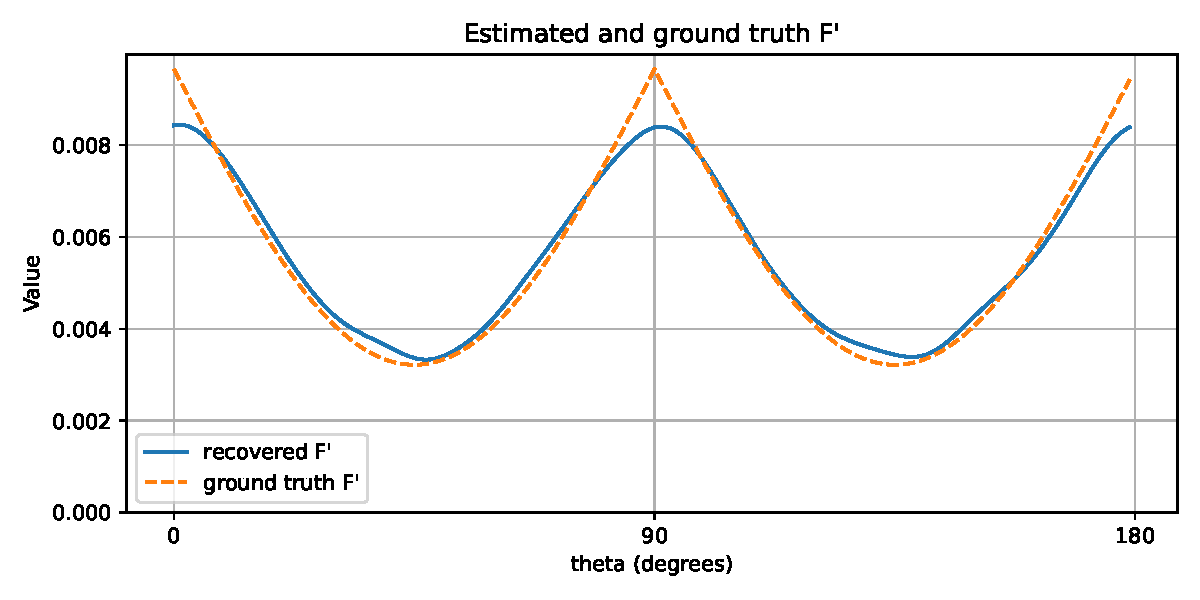
\includegraphics[width=\textwidth]{figures/recover_encoding.py_SimulateSynthetic_Parameterized_OtherNoiseLevels_Grid_VarySize.py_180_2_5_N40000_STEEPPERIODIC_STEEPPERIODIC.txt_180_4.0_6.0_Fprime.pdf}
  \end{minipage}



  \caption{
%Here, we provide an example of how to recover the encoding $\sqrt{J}(\theta)$ from simulated data, using Theorem 1.
%Results are shown in Figure~\ref{fig:recover-encoding}.
Here, we provide an example of how to recover the encoding $\sqrt{J}(\theta)$ from simulated data, using Theorem 1.
Recovering the encoding using Theorem 1, at four different levels of sensory noise. 40K trials were simulated, separately at each noise level, with $p=2$ and a periodic prior. We compute the empirical probability
$P=P\bigl(\hat{\theta}(\theta+\tfrac{h}{2})>\hat{\theta}(\theta-\tfrac{h}{2})\bigr)$ and then put
$\sqrt{J}(\theta)=\frac{\bigl(P-0.5\bigr)\sqrt{4\pi}}{h\,\Delta\theta}$ with $h=2^\circ$ (of the orientation space [$0^\circ$,$180^\circ$]) as an estimate of the derivative.
The result is convolved with a Gaussian kernel with $\sigma=6^\circ$.
}\label{fig:recover-encoding}
\end{figure}

\begin{comment}

python3 recover_encoding.py 180 4.0 6.0 SimulateSynthetic_Parameterized_OtherNoiseLevels_Grid_VarySize.py_180_2_2_N40000_STEEPPERIODIC_STEEPPERIODIC.txt
python3 recover_encoding.py 180 4.0 6.0 SimulateSynthetic_Parameterized_OtherNoiseLevels_Grid_VarySize.py_180_2_3_N40000_STEEPPERIODIC_STEEPPERIODIC.txt
python3 recover_encoding.py 180 4.0 6.0 SimulateSynthetic_Parameterized_OtherNoiseLevels_Grid_VarySize.py_180_2_4_N40000_STEEPPERIODIC_STEEPPERIODIC.txt
python3 recover_encoding.py 180 4.0 6.0 SimulateSynthetic_Parameterized_OtherNoiseLevels_Grid_VarySize.py_180_2_5_N40000_STEEPPERIODIC_STEEPPERIODIC.txt
\end{comment}

\begin{comment}
# Other ones than can in principle be run

python3 recover_encoding.py 180 4.0 6.0 SimulateSynthetic_Parameterized_OtherNoiseLevels_Grid_VarySize.py_180_2_2_N40000_STEEPPERIODIC_STEEPPERIODIC.txt
python3 recover_encoding.py 180 4.0 6.0 SimulateSynthetic_Parameterized_OtherNoiseLevels_Grid_VarySize.py_180_2_2_N40000_STEEPPERIODIC_UNIFORM.txt  
python3 recover_encoding.py 180 4.0 6.0 SimulateSynthetic_Parameterized_OtherNoiseLevels_Grid_VarySize.py_180_2_2_N40000_UNIFORM_STEEPPERIODIC.txt

python3 recover_encoding.py 180 4.0 6.0 SimulateSynthetic_Parameterized_OtherNoiseLevels_Grid_VarySize.py_180_2_3_N40000_STEEPPERIODIC_STEEPPERIODIC.txt
python3 recover_encoding.py 180 4.0 6.0 SimulateSynthetic_Parameterized_OtherNoiseLevels_Grid_VarySize.py_180_2_3_N40000_STEEPPERIODIC_UNIFORM.txt
python3 recover_encoding.py 180 4.0 6.0 SimulateSynthetic_Parameterized_OtherNoiseLevels_Grid_VarySize.py_180_2_3_N40000_UNIFORM_STEEPPERIODIC.txt

python3 recover_encoding.py 180 4.0 6.0 SimulateSynthetic_Parameterized_OtherNoiseLevels_Grid_VarySize.py_180_2_4_N40000_STEEPPERIODIC_STEEPPERIODIC.txt
python3 recover_encoding.py 180 4.0 6.0 SimulateSynthetic_Parameterized_OtherNoiseLevels_Grid_VarySize.py_180_2_4_N40000_STEEPPERIODIC_UNIFORM.txt
python3 recover_encoding.py 180 4.0 6.0 SimulateSynthetic_Parameterized_OtherNoiseLevels_Grid_VarySize.py_180_2_4_N40000_UNIFORM_STEEPPERIODIC.txt

python3 recover_encoding.py 180 4.0 6.0 SimulateSynthetic_Parameterized_OtherNoiseLevels_Grid_VarySize.py_180_2_5_N40000_STEEPPERIODIC_STEEPPERIODIC.txt
python3 recover_encoding.py 180 4.0 6.0 SimulateSynthetic_Parameterized_OtherNoiseLevels_Grid_VarySize.py_180_2_5_N40000_STEEPPERIODIC_UNIFORM.txt
python3 recover_encoding.py 180 4.0 6.0 SimulateSynthetic_Parameterized_OtherNoiseLevels_Grid_VarySize.py_180_2_5_N40000_UNIFORM_STEEPPERIODIC.txt

\end{comment}


\end{document}
